\documentclass[12pt,fleqn]{article}\usepackage{../../common}
\begin{document}
Türevler ve Entegraller

Türev ve entegral kavramlarını teorik olarak nasıl açıklarız? Her iki kavram da
modern matematikte artık limitler üzerinden temsil ediliyor. Geometrik olarak
bakarsak, bir $f(x)$ fonksiyonu var diyelim, bu fonksiyona $P$ noktasında
teğet olan sekant çizgisi olsun [1],

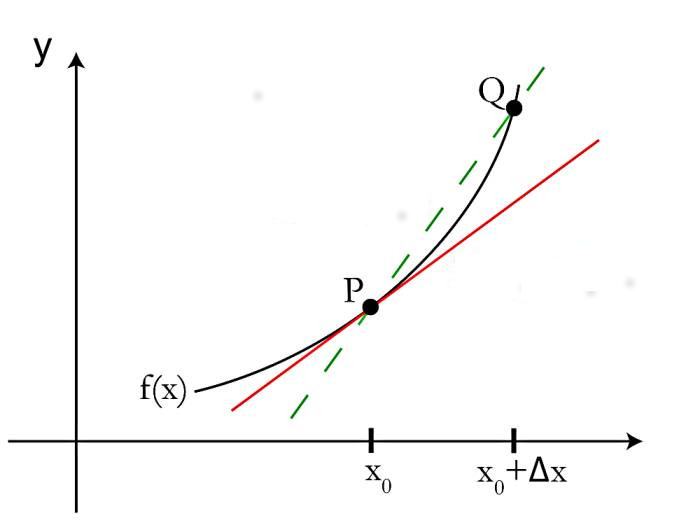
\includegraphics[width=15em]{ode_mattuck_65_diffint1_01.jpg}

Bu çizgi üzerinde iki nokta seçelim, $P,Q$'ya tekabül eden x ekseni üzerinde
biri $x_0$'da diğeri $x_0 + \Delta x$ üzerinde. Bu bölgeye yakından bakarsak,

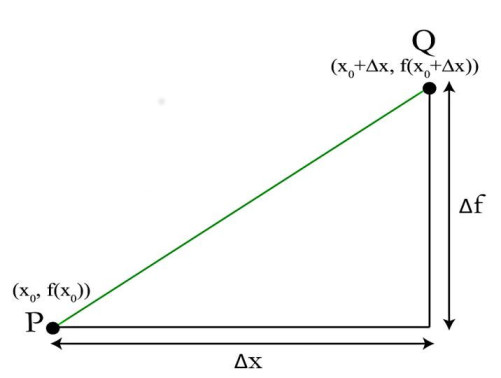
\includegraphics[width=15em]{ode_mattuck_65_diffint1_02.jpg}

$f'(x_0)$'nin, yani $x_0$ noktasında $f$'nin türevinin limitler üzerinden tanımı
şöyledir,

$$
\lim_{\Delta x \to 0} \frac{\Delta f}{\Delta x} =
\lim_{\Delta x \to 0} \frac{f(x_0 + \Delta x) - f(x_0)}{\Delta x} =
f'(x_0)
$$

Giriş seviyesinde Calculus'tan bilinen üsteli bir azaltıp çarpım haline getirme
tekniğini hatırlarsak, mesela $f(x) = x^2$ ise $f'(x) = 2x$ gibi, bu tekniği
limitler ile türetebiliriz. Genel bir $x^n$ için türetelim, aradığımız oran
şudur,

$$
\frac{\Delta f}{\Delta x} = \frac{(x_0-\Delta x)^n - x_0^n}{\Delta x}
\mlabel{1}
$$

Son ifadede $x_0$ yerine $x$ kullandık, notasyonu basitleştirmek için. Devam
edelim, $(x+\Delta x)^n$ nedir? Genel bir $(p + q)^n$ için düşünürsek,

$$
(p+q)^2 = p^2 + 2pq + q^2
$$

$$
(p+q)^3 = p^3 + 3 p^2 q + 3pq^2 + q^3
$$

$$
(p+q)^4 = p^4 + 4p^3 q + 6p^2 q^2 + 4p q^3 + q^4
$$

gibi devam edecektir.. Nihai formül için Binom Teorisi konusuna bakılabilir [3].
Fakat eldeki formüllerde bile bir kalıp farkedebiliyoruz, bu kalıp

$$
(p+q)^n = p^n + n p^{n-1} q + O(q^2) + q^n
$$

olarak ifade edilebilir. $O(q^2)$ olarak gösterilen ``$q^2$ ve üstü derecesini
içeren terimlerin toplamı'' notasyonudur. Bu tür bir gruplamak yapmak bize limit
alırken faydalı olacak. Problemimize uygularsak,

$$
(x+\Delta x)^n = x^n + n (\Delta x)x^{n-1} + O(\Delta x^2)
$$

Bu ifadeyi (1) içine koyalım,

$$
\frac{\Delta f}{\Delta x} =
\frac{x^n + n (\Delta x)x^{n-1} + O(\Delta x^2) - x^n}{\Delta x}
$$

$x^n$'ler iptal olacaktır, $\Delta x$ ile böldükten sonra

$$
= n x^{n-1} + O(\Delta x) - \frac{x^n}{\Delta x}
$$

Üstteki ifadenin limitini alınca $\Delta x$ içeren ifadeler yokolur,

$$
\lim_{\Delta x \to 0} \frac{\Delta f}{\Delta x} =
n x^{n-1}
$$

Yani

$$
\frac{\ud }{\ud x} x^n = n x^{n-1}
$$

Her türlü fonksiyon için limit yaklaşımı kullanılabilir, mesela $\sin(x)$ örneği
[4]'te işlendi.

Kaynaklar

[1] Jerison, {\em 18.01 Single Variable Calculus, Fall 2006},
    \url{https://ocw.mit.edu/courses/18-01-single-variable-calculus-fall-2006}

[2] Courant, {\em Introduction to Calculus and Analysis, Volume 1}

[3] Wikipedia, {\em Binomial Theorem},
    \url{https://en.wikipedia.org/wiki/Binomial_theorem}

[4] Bayramli, {\em Normal Diferansiyel Denklemler, Türevler ve Entegraller 2}
    
\end{document}
